\documentclass{article}

\usepackage{graphicx}
\usepackage{natbib}
\usepackage{amsmath}
\usepackage{hyperref}

\newcommand{\urlGammaCat}{\url{https://github.com/gammapy/gamma-cat}}

\title{GPS sky model for CTA 1DC}

\author{
  Zanin, Roberta
  \and
  Deil, Christoph
  \and
  Christofari, Pierre
}

%\date{\today} % Date for the report

\begin{document}

\maketitle

\begin{center}
\begin{tabular}{lr}
Status: & Work in progress \\
Version: & \date{\today} \\
Repository: & \url{https://github.com/gammasky/cta-dc} \\
\end{tabular}
\end{center}

\begin{abstract}
Abstract text
\end{abstract}

\section{Introduction}

What is this?

TODO: for which datasets was this model used? GPS, GC, EGAL?

\section{Sky model components}

\subsection{Known bright sources}

\subsubsection{gamma-cat}

We use gamma-cat (\urlGammaCat) for most known VHE sources,
except the ones listed in sections TODO and table TODO.

\subsubsection{Image sources}

See sky\_model/image\_sources

\subsubsection{Binaries}

See \verb=sky_model/binaries= and Table~\ref{tab:binaries}.

\begin{table*}[t]
\caption{
%
Gamma-ray binaries.
%
}
\label{tab:binaries}
\centering
\begin{tabular}{lrr}
\hline
Source Name  & GLON & GLAT \\
             & deg & deg \\
\hline
LS 5039      & 16.902 & -1.278 \\
PSR B1259-63 & 304.186 & -0.987 \\
\hline
\end{tabular}
\end{table*}

\subsection{Synthetic populations of faint sources}

\subsubsection{Pulsar wind nebulae}

\subsubsection{Supernova remnants}

We rely on Monte Carlo methods to simulate the population of SNRs potentially detectable by CTA. 
We simulate the time and location of supernova explosions in the Galaxy, assuming a rate of 3 SN per century, and a spatial distribution described as in~\cite{faucher}. Two mechanisms, via four types of progenitors, are considered:~thermonuclear (type Ia) and core--collapse (types Ib/c, IIP, IIb). The relative rates and typical parameters associated to each type, such as the total supernova explosion energy, the velocity of the wind and the mass of the ejecta, are adopted as in~\cite{seo}, so that every simulated supernova is assigned a type and corresponding parameters. 
At the location of each supernova, the typical value of the interstellar medium (ISM) is derived from surveys of atomic and molecular hydrogen~\cite{H1,H2}. The evolution of the shock radius $R_{\rm sh}$ and velocity $u_{\rm sh}$ is computed using analytical and semi--analytical description of~\cite{chevalier,pz05}. 

Finally, the gamma--ray luminosity of each SNR is computed. The contribution of protons and electrons is taken into account. At the shock, the particles are assumed to be accelerated with a slope following a power--law in momentum $n(p) \propto p^{-\alpha}$, where $\alpha$ is treated as a parameter in the range $4.1 - 4.4$. At the shock, we assumed that a fraction $\xi_{\rm CR}$ of the ram pressure of the shock expanding through the ISM is converted into CRs, where $\xi_{\rm CR} \approx 0.1$, and the shock compression factor is $\sigma=4$.  
The distribution of CRs inside the SNR is computed by solving a transport equation and the structure of the interior of the SNR is derived by solving the gas continuity equation, as in~\cite{pz03,pz05}.
The maximum momentum reached by protons is computed by assuming that protons escape the shock when their diffusion length equates a fraction $\zeta \approx 0.1$ of the shock radius, adopting a Bohm diffusion coefficient, this leads to $p_{\max} \propto R_{\rm sh} u_{\rm sh} B_{\rm down}$, where $B_{\rm down}$ is the magnetic field downstream of the shock. In order to account for magnetic field amplification downstream of the shock, and without making any assumption on the type of mechanism involved in the amplification, we describe $B_{\rm down} = \sigma B_{0}\sqrt{({u_{\rm sh}}/{v_{\rm d}})^{2}+1}$, where $v_{\rm d}$ is explicited in~\cite{zirakashviliaharonian2010} .
The hadronic contribution to the gamma--ray spectrum is then calculated following the approach of~\cite{kelner2006}, weighted by a factor 1.8 to take into account nuclei heavier than hydrogen. 

We follow by computing the leptonic component. 
The spectrum of electrons is parametrized adopting the same spectral shape as protons $\propto p^{-\alpha}$, weighted by a factor $K_{\rm ep}$, for momenta $p$ < $p_{\rm break}$, where $p_{break}$ accounts for radiative losses. above $p_{\rm break}$ the electron spectrum steepens by one order and follows $\propto p^{-\alpha-1}$. The maximum momentum of electrons is reached when the synchrotron loss time is of the order of the acceleration rate. The gamma--ray luminosity from inverse Compton scattering of electrons on the cosmic microwave background is computed following the description proposed by~\cite{gould}.

The approach presented here is described more in detail in \cite{cristofari2013,cristofari2017} and was used to provide a statistical test for the SNR hypothesis of the origin of CRs. 



\subsubsection{Composites}

\subsection{Diffuse emission}

TODO: need short description of ISO and GAL diffuse emission components, no?

\section{Illustrations and Checks}

\subsection{Spatial distribution in the Galaxy}

Show and discuss X, Y, Z, distance distribution of sources in the Galaxy.

\subsection{Spatial distribution on the Sky}

Show and discuss GLON, GLAT distribution

\subsection{Source sizes}

Do physical and observed size together here should be OK?

\subsection{Source fluxes}

Look at one or more integral flux measures.

Discuss CTA sensitivity and which sources might be visible here or later?

\subsection{Source spectra}

Just as an example: For PWN spectra, see Fig.~\ref{fig:pwn_spec}

\begin{figure}[t]
\begin{center}
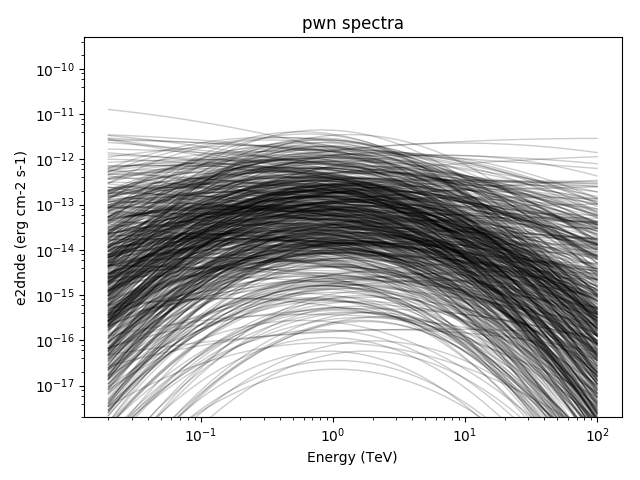
\includegraphics[width=1.0\textwidth]
{../sky_model_checks/ctadc_skymodel_gps_sources_spectra_pwn}
\caption{PWN spectra (just as an example of a Figure)}
\label{fig:pwn_spec}
\end{center}
\end{figure}


How do we compare to HGPS \citep{2013arXiv1307.4868C}?

\section{Conclusions}

How did we do? What can be done better in DC2?


\bibliographystyle{apalike}

\bibliography{cta_1dc_gps_sky_model}

\end{document}
